\documentclass[../../main.tex]{subfiles}
\begin{document}
\begin{appendices}
\crefalias{chapter}{appsec} % changes the name to appendix when \cref is used
%
\begin{comment}
    In this chapter we will focus on the techniques necessary to go from a analytical representation of a problem and constructing a numerical approach in order to solve it. A compromise must be made between accurate results and the time frame required to achieve them.   
\end{comment}
%    
\chapter{Integration Method}\label{app: Integration Method}
    Compared to established techniques for solving deterministic equations of motion, the methods for solving stochastic equations are a great deal less developed. 
    
    The most straightforward algorithm is based on the first-order Euler method for ordinary differential equations. Unfortunately, it requires a very small time step to produce sufficiently accurate results, making it highly inefficient \cite{ermakComputerSimulationCharged1975, ermakBrownianDynamicsHydrodynamic1978}. We opt for a Runge-Kutta based algorithm with added stochastic terms. Despite the greater complexity, by requiring more than one evaluation of the force acting upon each particle at a given moment, we can achieve comparable results with a significant larger time step, thus reducing significantly the computing time required.
            
    Consider \cref{eq: eg. langevin}, a form of the Langevin equation used throughout this work.
        \begin{equation}\label{eq: eg. langevin}
            \zeta\frac{d\mathbf{r}}{dt} = \mathbf{f}+\bm{\xi} \,,
        \end{equation}
    where $\zeta\ddfrac{d\mathbf{r}}{dt}$ is the viscous force, $\mathbf{f}$ is some external force and $\bm{\xi}$ gives the thermal noise. We discretize \cref{eq: eg. langevin} as follows
        \begin{equation}\label{eq: eg. discretized}
        \begin{gathered}
            \mathbf{r}(t + \Delta t) =  \mathbf{r}(t) + \ddfrac{\Delta t}{\zeta}\left\{\ddfrac{1}{2}\left[\mathbf{f}\left(\mathbf{r}(t)\right) + \mathbf{f}\left(\mathbf{r}^*(t + \Delta t)\right)\right] + \bm{\xi}\right\} \,, \\
            \mathbf{r}^*(t + \Delta t) =  \mathbf{r}(t) + \ddfrac{\Delta t}{\zeta}\left[\mathbf{f}\left(\mathbf{r}(t)\right) + \bm{\xi}\right] \,.
        \end{gathered}
        \end{equation}
    where $\bm{\xi}$ is one random number set by the computer with known mean and variance.
     
\chapter{Pseudo-Random Number Generator}\label{app: RNG}
    The force resulting from the collision of the fluid molecules with the Brownian particle, $\bm{\xi}$, is regarded as a stochastic variable with a Gaussian distribution.
    
    This creates a need to introduce randomness to our computer program. However, there is no trivial way to make a computer do something by chance, since, by definition, a computer is made to follow instructions and is, therefore, completely predictable. Instead, we make use of pseudo-random numbers.
    
    If we consider a function $f: S \rightarrow S$, where $S$ is a finite set of states, and an output function $g: S \rightarrow T$, where $T$ is the output space. We define
        \begin{equation}
            \begin{split}
                S_n &= f(S_{n-1}), \quad n \in \mathbb{N} \,,\\
                T_n &= g(S_n) \,,
            \end{split}
        \end{equation}
    and, by providing an initial value $S_0$ for the state, the seed, we can generate a sequence of numbers whose properties approximate, but are not equal to, the properties of sequences of truly random numbers.
    
    Pseudo-random number generators (PRNGs) are an efficient way of producing a large quantity of numbers in a short time, and even its deterministic nature can be useful for it allows to reproduce a certain sequence of numbers, and by implication, a certain experiment, if the seed is known. Unfortunately, PRNGs are also periodic. By using a finite state space, at some point a previous state will be reached and the sequence will repeat itself. This is far from a desirable characteristic but the majority of modern PRNGs have a period long enough that it can be ignored for most practical purposes.
    
    Despite this, the output from many commonly used PRNGs exhibit artefacts that cause them to fail many statistical pattern-detection tests, with shorter periods for some seed states, non uniform distributions and correlation of consecutive values, among others.
    
    In this work, the Mersenne Twister method is used \cite{matsumotoMersenneTwister623dimensionally1998}. Although not without some flaws, as it is neither particularly fast nor space efficient, it passes most statistical tests, with a large period which, combined with its straightforward implementation in C++, makes it a good choice for the application in question.

\chapter{Truncated Normal Distribution}\label{app: Dist Trunc}   
    Consider the standard normal distribution, where the probability distribution function of a random variable $X$ is given by
        \begin{equation}\label{eq: Truncated Distribution - pdf Normal}
            \phi_X(x) = a_X\exp \left( -\frac{x^2}{2} \right) \,,
        \end{equation}
    with $a_X = 1/\sqrt{2\pi}$ and $x\in\, \left] -\infty, +\infty \right[$. 
    
    We introduce a new random variable $Y$, based on the previous distribution but truncated at $\left|Y\right| < t $, This will have the following distribution
        \begin{equation}\label{eq: Truncated Distribution - pdf trunc without correction}
            f_Y(y) =
            \begin{cases}
                a_Y\exp \left( -\ddfrac{y^2}{2} \right) \quad &\text{if}\, \left| y \right| < t \\
                0 \quad &\text{if}\, \left| y \right| > t 
            \end{cases}
            \,,
        \end{equation}
    where normalisation requires that
        \begin{equation}\label{eq: Truncated Distribution - a_Y}
            a_Y = \ddfrac{1}{ \bigintssss_{-t}^t\exp \left( -\frac{y^2}{2} \right)} \,.
        \end{equation}
    The variance of this new distribution is given by
        \begin{equation}\label{eq: Truncated Distribution - var_Y}
        \begin{split}
            \sigma_Y^2 &= \bigintssss_{-t}^{t} y^2f_Y(y)\,dy = \\
            &= \frac{-2t \cdot \exp\left( -\ddfrac{t^2}{2} \right) + \sqrt{\ddfrac{\pi}{2}} \erf\left( \ddfrac{t}{\sqrt{2}} \right) - \sqrt{\ddfrac{\pi}{2}} \erf\left( -\ddfrac{t}{\sqrt{2}} \right)}{\sqrt{\ddfrac{\pi}{2}} \erf\left( \ddfrac{t}{\sqrt{2}} \right) - \sqrt{\ddfrac{\pi}{2}} \erf\left( -\ddfrac{t}{\sqrt{2}} \right)} \,.
        \end{split}
        \end{equation}
        
    Suppose we want to keep the variance equal to that of the non-truncated distribution. To do that, we redefine our random variable, $Y$, as $Z = c \cdot Y$. The probability density function of $Z$ is now
        \begin{equation}\label{eq: Truncated Distribution - pdf trunc with correction}
            f_Z(z) =
            \begin{cases}
                a_Z\exp \left( -\ddfrac{z^2}{2c^2} \right) \quad &\text{if}\, \left| z \right| < t \cdot c \\
                0 \quad &\text{if}\, \left| z \right| > t \cdot c 
            \end{cases}
            \,,
        \end{equation}
    with $a_Z = a_Y/c$.
    
    By definition we have that 
        \begin{equation}\label{eq: Truncated Distribution - c}
            \sigma_Z^2 = c^2 \sigma_Y^2 \Leftrightarrow c = \frac{\sigma_Z}{\sigma_Y} \,,
        \end{equation}
    leaving us only with the choice of a suitable value for $t$.
    
        \begin{figure}
            \centering
            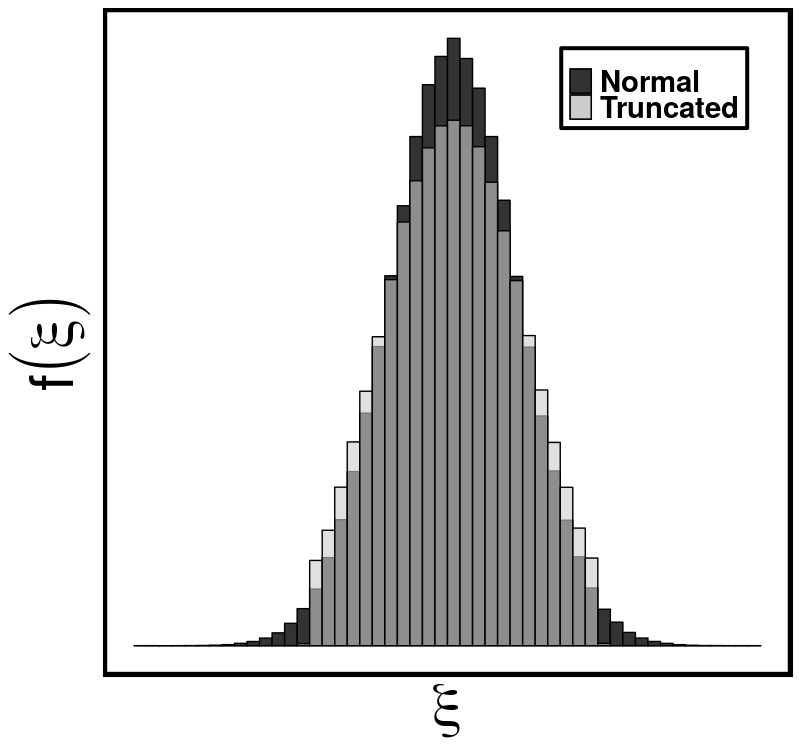
\includegraphics[scale=0.4]{Figures/truncated.png}
            \caption{Comparison between a normal distribution and its truncated version. We chose $\sigma_X = 4$, with $t = 2\sigma_X$. Note that the truncated version appears flatter. As we narrow the output interval, in other words as $\left| z \right|$ becomes smaller, the distribution becomes ever more flat, approaching a uniform one.}
            \label{fig: truncated dist}
        \end{figure}



\chapter{Pair Potential}\label{app: Pair Potential}
\section{Cut-Off Distance}\label{app: Potential Cutt-off}

    In the course of our simulation, one of the most time consuming tasks will be the calculation of the forces between inter-chain interacting pairs. Since a short ranged potential is used, after a certain distance the contribution of the force acting on the particle is negligible and doing that calculation amounts to nothing more than wasted time. 
    
    To avoid unnecessary calculations, we simply set a cut-off distance, $r_c$, above which the interaction is neglected. This creates a jump discontinuity at $r_c$, so the potential must be shifted upwards ensuring that $u(r_c) = 0$,
        \begin{equation}
            u(r_{ij}) = 
            \begin{cases}
                u(r_{ij}) - u(r_c) \quad &\text{if} \, r_{ij} < r_c \\
                0 \quad \quad &\text{if} \, r_{ij} \leq r_c \\
            \end{cases}
            \,.
        \end{equation}
    This is not yet sufficient for there is a discontinuity in the force calculation when $r=r_c$. We solve this by subtracting the derivative of the function on the point which guarantees that we arrive at a smooth function
        \begin{equation}
            u(r_{ij}) = 
            \begin{cases}
                u(r_{ij}) - u(r_c) - \frac{\partial u}{\partial t}\Bigr|_{\substack{r=r_c}}(r - r_c) \quad &\text{if} \, r_{ij} < r_c \\
                0 \quad &\text{if} \, r_{ij} \leq r_c\\
            \end{cases}
            \,.
        \end{equation}

\section{Reduced Units}\label{app: Reduced Units}
    When doing computer simulations, we are obliged to work in dimensionless or reduced units. By working with appropriate reduced units, where most numerical values will be the order of unity, we are able to avoid truncation and rounding errors that would be common if we were dealing with SI units at these scales. Setting up the model like this will also make it possible to re-scale it in order to describe a wider range of problems since any property can be scaled back to the appropriate physical units. 
    
    Since the particles in our system interact via a simple pair potential they can be completely specified through very few parameters such as $m$, $\sigma$ and $\epsilon$. From this definition, the units of every other physical properties can be re-scaled (\cref{tab: Reduced Units}) \cite{allenComputerSimulationLiquids2017}.
    
    To better understand this, consider the reduced time, $t$, which is simply the time, $t^*$, in reduced units. We start with the product of our three constants, each one raised to an arbitrary power,
    \begin{equation}\label{eq: Reduced Units - I}
        C = \sigma^a \epsilon^b m^c \,.
    \end{equation}
    Noting the units of this combination are
        \begin{equation}
                m^a J^b kg^c = m^a \left(kg \frac{m^2}{s^2}\right)^b kg^c = m^{a+2b} kg^{b+c} s^{-2b}\,,
        \end{equation}
    and that our time, $t^*$, in SI units is given in seconds, $s$, we have
        \begin{equation}
            m^{a+2b} kg^{b+c} s^{-2b} = s^1
        \end{equation}
    where it follows that $a = 1$, $b = -1/2$ and $c = 1/2$. Remembering \cref{eq: Reduced Units - I}, we can know write the reduced time as
        \begin{equation}
            t = \frac{t}{C} = t^* \left( \ddfrac{\sigma^2m}{\epsilon} \right)^{-\frac{1}{2}}\,.
        \end{equation}
%%%%%%
    \begin{table}[h]
        \centering
        \caption{A few examples of re-scaled properties. We chose to define our SI unit properties with the '*' in order to avoid confusion when they appear in the main body of this work.}
        \begin{tabular}{ || c | c || }
            \hline
    	        \textbf{Property} & \textbf{Reduced Units} \\ \hline
    	        Distance ($r$) &  $\ddfrac{r^*}{\sigma}$ \\ \hline
    	        Energy ($U$) & $\ddfrac{U^*}{\epsilon}$ \\ \hline
    	        Force ($f$) & $\ddfrac{f^*\sigma}{\epsilon}$ \\ \hline
    	        Mass ($m$) & $1$ \\ \hline
    	        Temperature ($T$) & $\ddfrac{k_B T^*}{\epsilon}$ \\ \hline
    	        Time ($t$) & $t^* \left( \ddfrac{\sigma^2m}{\epsilon} \right)^{-\frac{1}{2}}$ \\ \hline
        \end{tabular} 
        \label{tab: Reduced Units}
    \end{table}


    
    
\section{Periodic Boundary Conditions and Minimum Image Convention}\label{app: PBC & MIC}
    The behaviour of a finite system such is the one we are simulating is very different from one that is, for all intents and purposes, infinite (thermodynamic limit). So, in order to accurately describe our system, and minimise surface effects, we implement periodic boundary conditions. 
   
    To do that, we surround our simulation box with images of itself. In the course of our simulations, the motion of a particle in the central box is replicated in the neighbouring boxes. This ensures that if something leaves the central box, it's image will re-enter through the opposite side, and focus will shift to it, resulting in the conservation of density in the central box (and hence in the entire system).
   
    A consequence of defining such a system, is in the way we measure the distance between two pairs of particles. We can no longer see the central box as the only domain, but consider instead, the closest distance while accounting for all the created images (minimum image convention).
   
    Even though this is a simple premise, and a code can be easily thought to ensure this rules are followed, attention is still required, to avoid finite-size effects from poorly chosen system size, and to perform such calculations in the most efficient way possible, since that will be required a great many deal of times. However, this will depend on many factors such as the language in which the code is written or even on the hardware it's running. We settled for a simple conditional clause
%%%%%%%%%%%%%%%%%%%%%%%%%%%%%%%%%%%% 
\newpage
        \begin{minted}
        [
            mathescape,
            linenos,
            numbersep=5pt,
            gobble=2,
            frame=lines,
            framesep=2mm
        ]
        {cpp}
        /*      
                    **** Minimum Image Convention ****
        r: distance between particles
        L: Box Length
        half_L: L/2.0
        
        */
        
        inline void nic(double& r, const double& L, const double& half_L){
            if(r > half_L){
                r -= L;
            }
            else if(x < half_L){
                r += L;
            }
        }
        
        /*      
                    **** Periodic Boundary Condition ****
        r: distance between particles
        L: Box Length
        
        */
        
        inline void pbc(double& r, const double& BoxLength){
            if(r < 0){
                r -= L;
            }
            else if(x > L){
                r += L;
            }
        }
        
        \end{minted}
%%%%%%%%%%%%%%%%%%%%%%%%%%%%%%%%%%%%%%%    
\chapter{Some Integrals and ODEs}
\section{First-Order Linear Ordinary Differential Equations}\label{app: 1st ODE}
    This type of equations take the form of
        \begin{equation}\label{eq: 1st ODE}
            y'(t) + a(t)y(t) = b(t) \,,
        \end{equation}
    with $a(t)$ and $b(t)$ being continuous functions in the interval $I$. In order to solve \cref{eq: 1st ODE}, we make use of an integrating factor. We look for the antiderivative of $a(t)$, $A(t)$, and by multiplying both sides of \cref{eq: 1st ODE} by $\exp\left( A(t) \right)$ we get
        \begin{equation}
            \left( y(t) \exp\left( A(t) \right) \right)' = b(t) \exp\left( A(t) \right) \,.
        \end{equation}
    Integrating both sides reveals
        \begin{equation}
            y(t)  = \exp\left( -A(t) \right) \left( \bigintssss b(t) \exp\left( A(t) \right) dt \right) \,, \quad t \: \in \: I \,,
        \end{equation}
    where in $\bigintssss b(t) \exp\left( A(t) \right) dt$ we have an arbitrary constant $C \,\in\, \mathbb{R}$, determined if an initial condition, $y(t_0) = y$ with $t_0 \,\in\, I$, is provided.
    
\section{Gaussian Integral}\label{app: Gaussian Int}
    The formula for the Gaussian integral is
        \begin{equation}
            \bigintsss_{-\infty}^{+\infty} \exp (-ax^2 + bx) = \left( \frac{\pi}{a}\right)^\frac{1}{2}\exp\left( \frac{b^2}{4a} \right)
        \end{equation}
    where $a$ is a positive constant and $b$ is an arbitrary complex variable.

\end{appendices}
%        
\end{document}